\documentclass[10pt, a4paper, conference]{IEEEtran}
\usepackage{graphicx}
\title{Project Proposal: Efficient Message Passing}                            
\author{
	\IEEEauthorblockN{Stephen I. Roberts}
	\IEEEauthorblockA{Department of Computer Science\\
					 The University of Warwick}
} 
\date{}
\hyphenation{scaling}
\begin{document}                                                                
\maketitle                                                                    

\section{Background}

Stencil codes are commonly found in applications where computer simulation is used to model physical processes. These applications employ iterative kernels which traverse elements of the simulation and update them based on the values of their neighbours. The pattern of neighbourhood cells which provide input to each update, such as the one seen in \figurename~\ref{fig:von_neumann_stencil}, is referred to as a stencil.

\begin{figure} 
\centering 
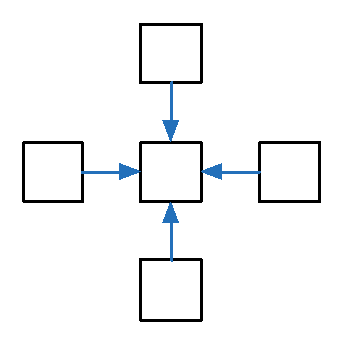
\includegraphics[width=2.5in]{graphics/2d_von_neumann_stencil.pdf}
    \caption{4 point 2D von Neumann style stencil}
    \label{fig:von_neumann_stencil}
\end{figure} 

Scientific computing workloads are typically spread over multiple nodes within a cluster to reduce time to solution and allow larger simulation domains. For stencil codes, the simplest approach is to statically assign each node with a fixed-size continuous subsection of the simulation domain. Nodes then only have to communicate with their neighbours to exchange boundary data at the end of each simulation step.

\begin{figure} 
\centering 
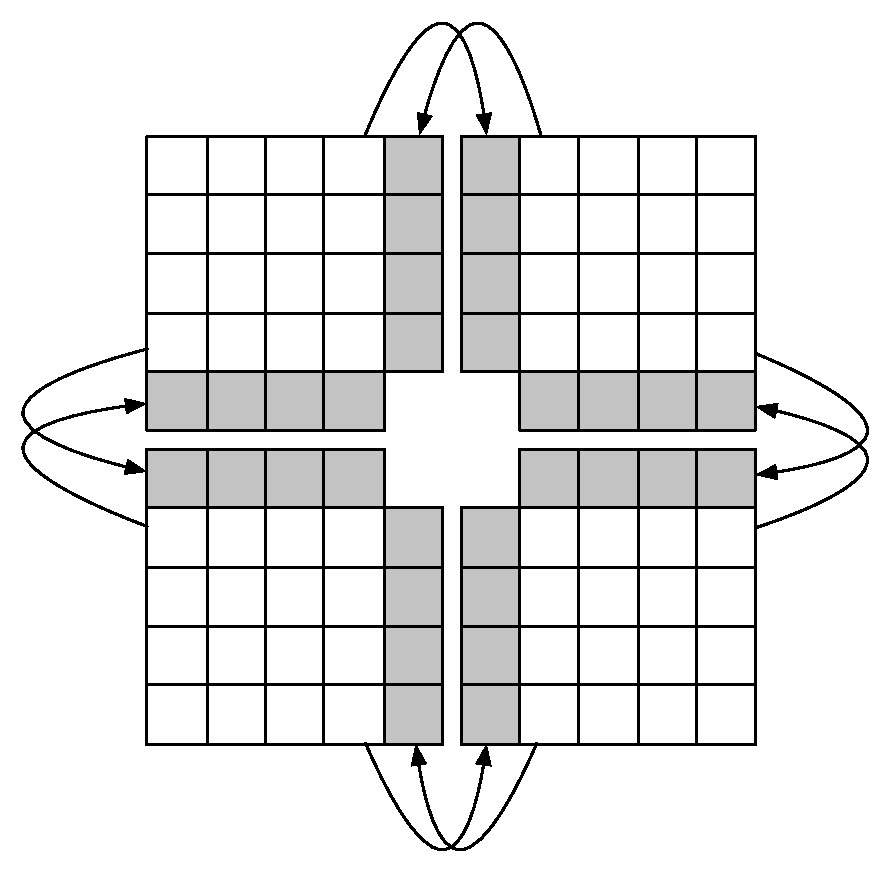
\includegraphics[width=2.5in]{graphics/2d2x2comms.pdf}
    \caption{Communications patterns in 2D decomposition over 4 nodes.}
    \label{fig:2dcp}
\end{figure}

\figurename~\ref{fig:2dcp} shows how ghost cells can be used in two dimensions to support boundary communications. The ghost cells mirror the current values in the boundary cells of their corresponding neighbour processor. Once boundary cells are swapped each node can perform its time step calculations independently.


\begin{figure} 
\centering 

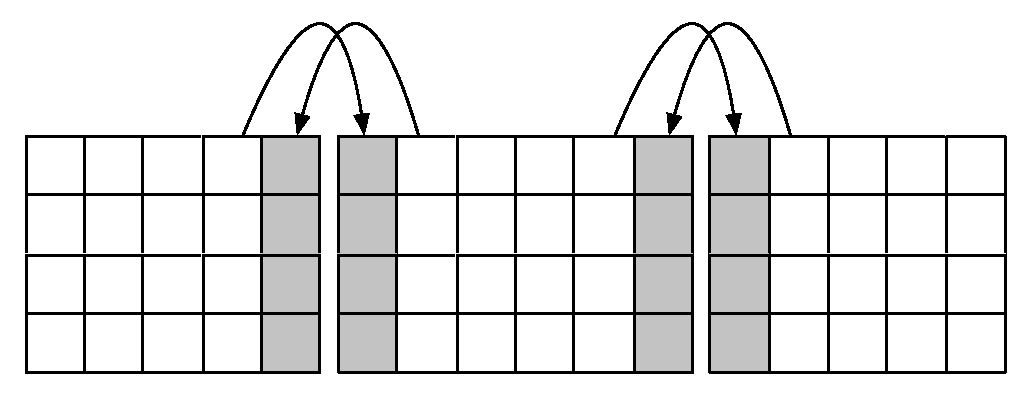
\includegraphics[width=2.5in]{graphics/1d3x1comms.pdf}
    \caption{Communications patterns in 1D decomposition.}
    \label{fig:1dcp}
\end{figure}






Lorem ipsum dolor sit amet, consectetur adipiscing elit. Curabitur ultricies est eget massa pulvinar ultrices. In id erat at odio malesuada posuere non nec tellus. Sed lacinia elit ac magna sagittis, at pellentesque urna sodales. Sed pharetra consequat nisi vitae egestas. Cras elementum tristique nunc vel rhoncus. Aenean iaculis magna ut diam tempus hendrerit. Donec pellentesque sodales dui id semper.

Praesent tincidunt arcu ac turpis volutpat tristique. Suspendisse faucibus tempor velit, condimentum facilisis urna varius sit amet. Curabitur ipsum arcu, ultricies nec gravida ac, pretium id nunc. Curabitur molestie orci ipsum, nec aliquam dui sollicitudin vel. Sed nec congue leo, ut consectetur nulla. Ut laoreet rutrum metus, ac pharetra purus facilisis ut. Praesent elementum lacinia leo, sit amet lobortis elit fringilla a. Phasellus et nisl nec quam iaculis placerat vel vel augue. Duis sit amet volutpat lorem, in eleifend turpis. Morbi a mauris tincidunt massa scelerisque luctus ut in nibh. Nam faucibus tortor luctus, sagittis quam sit amet, feugiat risus.

Quisque tempus enim non velit vestibulum vestibulum. Fusce sollicitudin eleifend dui vel consequat. Nullam vitae auctor libero. Quisque a turpis suscipit, vestibulum leo iaculis, aliquam lacus. Proin nec ligula arcu. Pellentesque facilisis scelerisque risus, ac cursus odio vehicula ac. Nam nibh dolor, feugiat in pulvinar venenatis, malesuada nec dui. Sed metus leo, volutpat nec velit nec, elementum gravida erat. In iaculis tincidunt felis ac laoreet.

Nunc fermentum ullamcorper ipsum ac rhoncus. Fusce et nibh odio. Suspendisse sit amet laoreet turpis. Donec neque nisl, faucibus et orci pulvinar, tristique tincidunt nisi. Aliquam rutrum tortor ac feugiat facilisis. Sed ultricies euismod euismod. Sed tincidunt iaculis turpis, ac sodales tellus sagittis ac. Morbi a tortor neque. Praesent posuere vestibulum nisi, id gravida orci suscipit a. Maecenas egestas sem vel ullamcorper pellentesque.

Morbi dictum ligula eu leo faucibus adipiscing id et neque. Sed rutrum lectus sit amet velit laoreet sollicitudin. Praesent porta cursus erat, et auctor tellus dapibus ac. Etiam et lacus quis leo feugiat vulputate et in libero. Nullam auctor lectus sit amet dolor laoreet gravida. Mauris molestie et nunc sit amet facilisis. Sed scelerisque nec metus id pellentesque. Class aptent taciti sociosqu ad litora torquent per conubia nostra, per inceptos himenaeos. Donec eget ipsum eu enim rutrum malesuada vel sit amet quam. Proin ut dui erat. Nulla fermentum non augue vitae malesuada. Sed suscipit justo at mollis mattis. Suspendisse potenti.






\end{document}